\chapter[INTRODUCTION AND LITERATURE REVIEW]{INTRODUCTION AND \\  LITERATURE REVIEW}

\section{Author's Message}

Howdy! This is my honor to organize the LATEX Thesis Template for Texas A\&M
University
\footnote{This is a test to see how the footnote is displayed in long text below the main content. The font size is 10pt if you don't modify the default setting. As you can see, it is single space.} 
as a graduate student at ECE under the guidance of OGAPS@TAMU. I have
 applied \LaTeX ~ to write my bachelor and master thesis in English previously. My approach is to deal with all the questions/settings with high level package or
global settings. Please send me an email at shray\_sharan@exchange.tamu.edu if you have any questions about the thesis template.



\subsection{Brief Usage of the Template}

some text here


\subsection*{Software to Install}

\textbf{MikTeX} or \textbf{ProTeXt} is the free software recommended for Windows PC users to
compile your \LaTeX ~ document. To compile for this document, XeLaTeX compiling engine
is used. Another software called \textbf{JabRef} is also recommended for bibliography/reference
management, its usage is similar with EndNote under Office Word.

\subsection*{Procedure to Compile LATEX Document}


some text here


\subsection{How to Fill this Document}
The document structure is organized in the main .tex file, TAMUthesis\_Template.tex,
which has the same name as the output PDF file. Content in each chapter is under the
folder of data. You can open the .tex files under the data folder to modify. Four chapters
are added initially. To add in more chapters into the LATEX document, please open the
TAMUthesis\_Template.tex files and goto line No. 280 as shown in Figure \ref{fig:addMoreChapters}.
For the rest of the document, you can just delete the content in the data folder and
fill your documents and then compile under TAMUthesis\_Template.tex.)

\subsection{Reference Usage and Example}

This subsection test the usage of Reference. Paper \citet{McLoughlin:2014:SVA:2687082.2687090} 
is referred in this way. Actually,the option is available for you to change the default way how reference appears. The default and most commonly used option \cite{einstein} is displayed here.

\begin{figure}[ht]

\centering
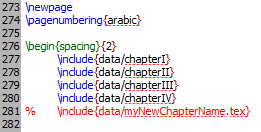
\includegraphics[scale=1.75]{TAMUthesis_AddChapter.png}
\caption[Add More Chapters into TAMUthesis\_Template.tex]{Add More Chapters into TAMUthesis\_Template.tex. For example, a new Chapter named "myNewChapterName.tex" is Created under the
folder of data.}



\label{fig:addMoreChapters}

\end{figure}


 


Unrelated citations are referred here for test of Reference Section only\cite{Andraka:1998:SCA:275107.275139}. If you
find the Reference \cite{Barrera:2013:APC:2482767.2482778} has more items than you need \cite{beritelli2002performance}.

\subsection{Equation Usage}

some text here

\subsection{Cover Page}

Some text here

\section{Specification in this TAMU Thesis \LaTeX ~ Template}

\subsection{Chapter Method Requirements}
 
some text here

\subsection{Subheadings Requirements}
some text here
 
 \subsection{Third-Order Subheadings}
 
some text here
 \section{Test Section}
 
 Test Content is displayed below.
 
 \section{Thesis Organization}
 
Example code below for \LaTeX ~  description environment. 
 
 \begin{description}
 \item[The 1st chapter] introduces the background.
 \item[The 2nd chapter]  briefly describes how to do it.
 \item[The 3rd chapter] details the design of the hardware. Test and verification of this hardware is located in Appendix A.
 \item[The 4th Chapter] issues the discussions and gives the summary.
 \item[The Appendix] contains some less-intersting, but still significant test benches, test setup details and test result information. It is provided in Appendix B. Appendix B.3 details
the usage.
 \end{description}
 

 






 


